\documentclass{article}

\usepackage{amsmath}
\usepackage{graphicx}

\title{Extracting Information from Star Forming Clumps: Temperature, Mass and Luminosity}
\date{2020-04-14}
\author{Morgan Langford}

\begin{document}
\pagenumbering{gobble}
\maketitle
\newpage
\pagenumbering{arabic}

\section{Introduction}
\subsection{Star Formation}
\paragraph{}
The interstellar medium (ISM), the space between the stars, has four components: matter, in the form of dust and gas; electromagnetic radiation; gravitational fields and magnetic fields (Kay, Palen, Smith, \& Blumenthal, 2013). It has a chemical composition of ~90\% Hydrogen, ~10\% Helium and only ~0.1\% more massive elements (Kay et al., 2013). ~99\% of interstellar matter is gaseous and it has an average density of $0.1 atoms/cm^3$. To give some point of reference, the air we breathe on Earth is about $2.7 x 10^{19} atoms/cm^3$ and the best vacuum we can create is still $10^{10} atoms/cm^3$. 

\begin{figure}[h!]
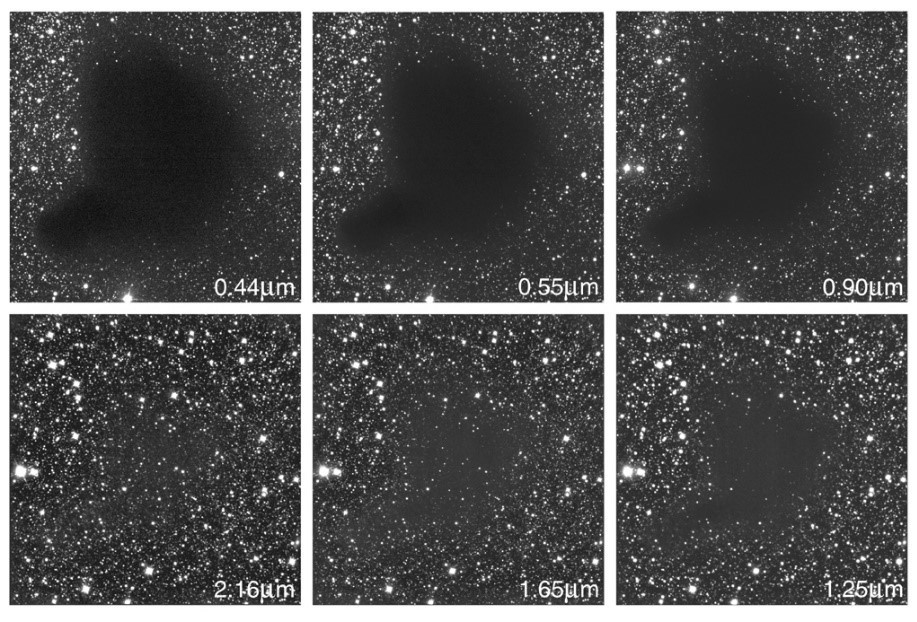
\includegraphics[width=\linewidth]{dust.jpg}
\caption{Images of the same cloud, taken at different wavelengths displaying 'interstellar extinction' (Walter, 1999)}
\label{fig:dust1}
\end{figure}

\paragraph{}
Interstellar dust makes up approximately 1\% of the material in the ISM. In size, it ranges from the size of a large molecule to ~300 nm across (Kay et al., 2013). Don’t be fooled by its size, however, as it is extremely good at blocking out light. This is known as interstellar extinction. It best blocks out light which has a wavelength about the size of the dust grain, meaning short wavelengths are absorbed or scattered whereas long wavelengths pass through, uninhibited (Bergin \& Tafalla, 2007). This effect is displayed in Figure \ref{fig:dust1}, showing the cloud quite visible at 0.44 µm and almost invisible at 2.16 µm, suggesting a large number of the dust grains are around 0.44 µm in size. 


\end{document}